\chapter{Experimental Evaluation and Discussion}
\label{chapter:evaluation}

This chapter presents the comprehensive empirical evaluation of the AILS-NTUA framework on the multi-turn conversational MTRAGEval benchmark (SemEval-2026 Task~8). We recap the model configuration and evaluation protocol (Section~\ref{sec:eval-setup}), quantify the individual contributions of retrieval and generation pipeline components through systematic ablation (Sections~\ref{sec:taskA-ablations}--\ref{sec:taskB-ablations}), analyze the end-to-end bottleneck, in which answerability calibration is the decisive factor under the test distribution (Section~\ref{sec:taskC-bottleneck}), and report the official, frozen leaderboard results (Section~\ref{sec:leaderboard}).

%==============================================================
\section{Experimental Setup and Baseline Benchmarking}
\label{sec:eval-setup}
%==============================================================

All architectural hyperparameter tuning and incremental component evaluations were conducted exclusively on the official MTRAG development set, comprising $110$ human-authored conversations across $842$ dialogue turns. Final evaluation was performed on the held-out evaluation test set, containing $507$ turns embedded within $507$ conversations---as established in Section~\ref{sec:key-challenges}, every test-set record consists of a \emph{single} evaluated turn drawn from a historical trace, and almost all of these turns ($465$ of $507$, $91.7\%$) are non-first turns that require contextual understanding, so the ``easy'' first-turn queries that inflate development-set averages are rare.

\subsection{Model Configuration Overview}
\label{sec:model-config-overview}

Before turning to the ablation results, we briefly recap the model assignment established under the capability-aligned routing principle of Section~5.3 (Table~\ref{tab:routing-en}): DeepSeek-V3.2 handles all five query rewriting strategies (Section~5.2.1) as well as span extraction and technical judging, GPT-4o is used for dual-candidate answer generation (Section~\ref{sec:generation-pipeline}) and for the three Task~C answerability judges (Section~\ref{sec:e2e-system}), and GPT-4o-mini covers the remaining lightweight, high-frequency stages (conversational triage, unanswerable-turn detection, user-satisfaction judging, and micro-adjustment). No component of the pipeline was fine-tuned on MTRAG data; all reported gains stem from prompt engineering and architectural design choices, evaluated exclusively on the development set unless otherwise noted.

\subsection{Hyperparameter Configuration}

Table~\ref{tab:hyperparams-en} consolidates the core hyperparameter values referenced throughout this chapter, all tuned exclusively on the development set and held fixed for the frozen test-set submission.

\begin{table}[h]
\centering
\small
\begin{tabular}{ll}
\toprule
\textbf{Parameter} & \textbf{Value} \\
\midrule
First-stage retrieval depth per reformulation ($N$) & 100 \\
Cross-encoder reranking depth ($k$) & 60 \\
Hybrid fusion weight ($\alpha$, Eq.~\eqref{eq:hybrid-rerank}) & 0.5 \\
Nested RRF internal smoothing ($k_{\text{internal}}$) & 40 \\
Task~A retrieved passages & 10 \\
Task~C retrieved passages & 3 \\
Extractiveness ideal band ($r_4$) & $[0.28, 0.38]$ \\
Answerability confidence threshold ($\tau$) & 0.7 \\
Dissenter override threshold ($\theta$) & 0.7 \\
User Satisfaction Judge invocation rate & $60\%$ \\
\bottomrule
\end{tabular}
\caption{Core system hyperparameters, tuned on the development set and frozen for test-set evaluation. Section~\ref{sec:taskC-bottleneck} discusses how this dev-only calibration may contribute to the Task~C performance gap.}
\label{tab:hyperparams-en}
\end{table}

%==============================================================
\section{Task A Retrieval Ablations and the Ensemble Paradox}
\label{sec:taskA-ablations}
%==============================================================

\subsection{Retriever Family Comparison}

Prior to any query rewriting, we benchmarked nine retrievers spanning lexical, dense, and learned sparse families on the full $777$-query development set. Table~\ref{tab:retriever-comparison-en} reports the outcome: ELSER~v1 substantially outperforms every alternative, exceeding the strongest dense competitor (Cohere Embed~v4) by $+8.6$ Recall@5 points and BM25 by $+33.0$ points on the same $777$ queries. This comparison must be read in light of how MTRAG was constructed: benchmark annotators primarily reviewed ELSER-retrieved passages when producing relevance judgments, so passages surfaced only by other retrievers are more likely to be unjudged and are scored as non-relevant. Part of ELSER's advantage may therefore reflect this pooling bias. We did not run a judged-only analysis that would quantify its size (see Section~\ref{sec:pooling-bias}).

\begin{table}[h]
\centering
\small
\begin{tabular}{llcc}
\toprule
\textbf{Type} & \textbf{Retriever} & \textbf{R@5} & \textbf{nDCG@5} \\
\midrule
Lexical & BM25 & 0.153 & 0.130 \\
\midrule
\multirow{5}{*}{Dense} & Cohere Embed v4 & 0.397 & 0.362 \\
& AWS Titan v1 & 0.352 & 0.328 \\
& Voyage-3.5-L & 0.321 & 0.302 \\
& GTE-Large & 0.326 & 0.293 \\
& BGE-Large-v1.5 & 0.282 & 0.251 \\
\midrule
\multirow{3}{*}{Sparse} & \textbf{ELSER v1} & \textbf{0.483} & \textbf{0.444} \\
& ELSER v2 & 0.411 & 0.380 \\
& SPLADE v3 & 0.402 & 0.374 \\
\bottomrule
\end{tabular}
\caption{Retriever comparison, $777$ development-set queries, no query rewriting. ELSER~v1 exceeds Cohere Embed~v4 by $+8.6$ R@5 points; see the text for the pooling-bias caveat.}
\label{tab:retriever-comparison-en}
\end{table}

A natural objection to Table~\ref{tab:retriever-comparison-en} is that ELSER's advantage could be an artifact of the downstream pipeline having been co-optimized around it, rather than an intrinsic retrieval quality difference. To rule this out, we additionally optimized each retriever \emph{independently}---applying the same multi-strategy rewriting and reranking components of Sections~\ref{subsec:rewriting-engine}--\ref{subsec:reranking} to each candidate retriever in turn---and compared the resulting recall at multiple cutoffs (Table~\ref{tab:retriever-optimized-en}). ELSER retains the best Recall@5/Recall@10 even after this independent optimization, indicating that its advantage is not an artifact of score-scale compatibility with the downstream fusion pipeline (the pooling-bias caveat of Section~\ref{sec:pooling-bias} still applies).

\begin{table}[h]
\centering
\small
\begin{tabular}{lcccc}
\toprule
\textbf{Retriever} & \textbf{R@5} & \textbf{R@10} & \textbf{R@50} & \textbf{R@100} \\
\midrule
\textbf{ELSER v1} & \textbf{0.607} & \textbf{0.729} & \textbf{0.873} & \textbf{0.901} \\
SPLADE & 0.539 & 0.657 & 0.836 & 0.874 \\
Cohere & 0.503 & 0.657 & 0.823 & 0.854 \\
BM25 & 0.444 & 0.536 & 0.688 & 0.735 \\
\bottomrule
\end{tabular}
\caption{Per-retriever recall after each retriever is independently optimized with the full rewriting and reranking pipeline. ELSER dominates at R@5/R@10 even under this controlled comparison.}
\label{tab:retriever-optimized-en}
\end{table}

\subsection{Incremental Value of Query Rewriting Strategies}

Table~\ref{tab:rewrite-ablation-en} documents the incremental performance improvement achieved by sequentially adding the five query rewriting strategies of Section~5.2.1 into the single-retriever index pool. Cumulative integration of all five strategies combined with Nested RRF yields Recall@5$=0.607$, a $+25.7\%$ relative improvement over the unaugmented baseline, in line with Hypothesis~H1. Two caveats apply to the reading of this table. First, its rows are cumulative, so each increment is conditional on the strategies already added and on the order in which they were added; a leave-one-out ablation was not performed. Second, the table does not isolate individual components of the retrieval configuration: it does not indicate where cross-encoder reranking enters the chain (its effect is reported separately in Table~\ref{tab:reranking-alone-en}), and a direct comparison between Nested RRF and a flat RRF over the same five inputs was not retained. The $+25.7\%$ figure should therefore be attributed to the complete retrieval configuration rather than to any single component.

\begin{table}[h]
\centering
\small
\begin{tabular}{lcc}
\toprule
\textbf{Retrieval Configuration} & \textbf{Recall@5} & \textbf{Relative Improvement} \\
\midrule
Unaugmented Baseline (Original Query) & 0.483 & --- \\
+ Minimal Rewrite & 0.527 & $+9.1\%$ \\
+ Corpus-Specific Expansion & 0.558 & $+15.5\%$ \\
+ Chain-of-Thought (CoT) Analysis & 0.573 & $+18.6\%$ \\
+ Hypothetical Document Embedding (HyDE) & 0.584 & $+20.9\%$ \\
+ Anchor Keyword Targeting & 0.591 & $+22.4\%$ \\
+ Nested RRF Fusion (Hierarchical Tree) & \textbf{0.607} & \textbf{$+25.7\%$} \\
\bottomrule
\end{tabular}
\caption{Incremental ablation of query rewriting strategies on the development set. Rows are cumulative. The largest single increment comes from Minimal rewriting ($+0.044$ R@5), followed by Corpus-Specific expansion ($+0.031$).}
\label{tab:rewrite-ablation-en}
\end{table}

Per-strategy analysis further reveals that no single reformulation dominates uniformly across domains: Corpus-Specific achieves the best single-strategy performance in ClapNQ ($R@5{=}0.637$) and FiQA ($R@5{=}0.491$), Chain-of-Thought leads in Govt ($R@5{=}0.580$), and Minimal is strongest in the technical Cloud domain ($R@5{=}0.463$). HyDE, notably, is the \emph{weakest} single strategy across all four domains, yet its inclusion in the full Nested RRF ensemble is not redundant: the complete five-strategy fusion ($R@5{=}0.607$) exceeds even the best individual strategy by $6.6$ points. Because the complete configuration also includes reranking (Table~\ref{tab:reranking-alone-en}), part of this difference may be due to the reranker; the comparison is therefore consistent with, but does not isolate, the \emph{complementarity} of the strategies.

\subsection{The Role of Reranking: Complementary, Not Substitutive}
\label{sec:reranking-role}

Table~\ref{tab:reranking-alone-en} isolates the specific contribution of cross-encoder reranking (Section~\ref{subsec:reranking}). Using a cross-encoder \emph{as the sole ranking mechanism}---bypassing the sparse retriever entirely---lowers Recall@5 by $4.6$--$10.6$ points ($8.7$--$20.0\%$ relative) compared with the ELSER baseline, despite the strong standalone benchmark performance of these same reranker models on static IR collections. Only the weighted RRF fusion of retriever and reranker signals (Equation~\eqref{eq:hybrid-rerank}) yields an improvement ($+0.067$ R@5, $+12.7\%$ relative)---an increment of the same order as the gains attributed to the additional rewriting strategies in Table~\ref{tab:rewrite-ablation-en}--- confirming that reranking functions as a complementary refinement filter over an already-relevant candidate pool rather than an independent source of retrieval quality.

\begin{table}[h]
\centering
\small
\begin{tabular}{lcc}
\toprule
\textbf{Configuration} & \textbf{Recall@5} & \textbf{$\Delta$ vs.\ baseline} \\
\midrule
ELSER v1 (baseline, with Minimal rewrite) & 0.527 & --- \\
Cohere Rerank v4 (sole ranking signal) & 0.481 & $-8.7\%$ \\
Voyage-Reranker-2.5 (sole ranking signal) & 0.469 & $-11.0\%$ \\
Cross-Encoder MS-MARCO (sole ranking signal) & 0.421 & $-20.0\%$ \\
\textbf{ELSER + Cohere, weighted RRF fusion} & \textbf{0.594} & \textbf{$+12.7\%$} \\
\bottomrule
\end{tabular}
\caption{Standalone reranking degrades performance; weighted RRF fusion with the sparse retriever yields complementary gains.}
\label{tab:reranking-alone-en}
\end{table}

We additionally investigated LLM-based reranking as a potential substitute for the fixed cross-encoder (Hypothesis~H4). Three formulations---pointwise scoring, listwise reordering in the style of RankGPT~\citep{sun2023rankgpt}, and generation-based ranking, all operating on the same top-$20$ candidate pool---were evaluated against the weighted RRF baseline of $R@10{=}0.725$. None improved upon this baseline when used as a substitute ranking signal: pointwise LLM scoring achieved $R@10{=}0.701$, listwise reordering $0.688$, and generation-based ranking $0.618$, at a substantially higher API cost than the weighted RRF fusion. Interpolating the LLM scores into the final ranking with a small fixed weight ($w \in [0.2, 0.45]$) instead yields only marginal gains (at most $+2$ percentage points in Recall@5 per domain). This result supports H4: once first-stage recall approaches saturation ($R@100 > 0.90$), general-purpose LLM judges lack the fine-grained discriminative sensitivity to replace a well-calibrated, purpose-built reranker, and the marginal benefit they provide as an auxiliary signal does not justify their added computational cost.

\subsection{Deconstructing the Retriever Ensemble Paradox}
\label{sec:ensemble-paradox}

A central finding of this thesis is that, under the official relevance judgments, heterogeneous multi-retriever ensembling does not help as a stabilization strategy once the single-retriever pipeline is optimized. Table~\ref{tab:ensemble-paradox-en} tracks this paradox across three stages of pipeline maturity: as the ELSER-only configuration improves through query rewriting (from $R@5{=}0.497$ with no rewriting\footnote{This early-stage run yields $R@5{=}0.497$ for ELSER~v1 without rewriting, slightly above the $0.483$ of Table~\ref{tab:retriever-comparison-en}. The two values come from separate experimental runs whose configurations we could not fully reconcile; the difference ($0.014$) does not affect the sign reversal reported here.} to $R@5{=}0.607$ with the full five-strategy ensemble), the \emph{marginal} benefit of adding alternative retrievers not only shrinks but reverses sign. At the early, unrewritten stage, adding all alternative retrievers improves $R@5$ from $0.497$ to $0.568$; at the fully optimized stage, the same addition \emph{degrades} $R@5$ from $0.607$ to $0.569$ on the same $777$ queries, even though $R@100$ continues to improve monotonically at every stage.

\begin{table}[h]
\centering
\small
\begin{tabular}{lccc}
\toprule
\textbf{Configuration} & \textbf{R@5} & \textbf{R@100} & \textbf{Unique golds / avg.\ rank} \\
\midrule
\multicolumn{4}{l}{\textit{Early Stage --- No Rewriting}} \\
ELSER v1 alone & 0.497 & 0.779 & --- \\
+ All alternative retrievers & 0.568 $\uparrow$ & 0.920 $\uparrow$ & 803 / 22.5 \\
\midrule
\multicolumn{4}{l}{\textit{Final Stage --- Optimized 5-Rewrite Ensemble}} \\
ELSER v1 alone & \textbf{0.607} & 0.901 & --- \\
+ All alternative retrievers & 0.569 $\downarrow$ & \textbf{0.926} $\uparrow$ & 141 / 39.5 \\
\bottomrule
\end{tabular}
\caption{The ensemble paradox: as the single-retriever pipeline matures through query rewriting, the marginal value of retriever ensembling reverses from positive to negative at $R@5$, even as it remains positive at $R@100$. Unique gold documents contributed by alternative retrievers settle at an average rank of $39.5$ after fusion (between $27.5$ and $54.2$ depending on the retriever)---below the top-$10$ cutoff used for Task~A scoring.}
\label{tab:ensemble-paradox-en}
\end{table}

A plausible mechanism for this reversal is the following: as the single-retriever configuration becomes increasingly precise at top-$k$, the unique gold documents that alternative retrievers contribute are, by construction, documents that ELSER did \emph{not} rank highly---and these settle at average ranks between $27.5$ (BM25) and $54.2$ (SPLADE) after fusion ($39.5$ for the full ensemble), well below the top-$10$ cutoff that determines Task~A scoring. Meanwhile, the act of fusing in a second, differently-calibrated ranking signal introduces noise that displaces borderline-relevant ELSER hits out of the top-$5$. This finding directly informs the architectural principle of Section~5.1: retrieval stability is better served by \emph{diversifying the query} against a single, well-aligned index than by \emph{diversifying the index} against a single query.

\paragraph{Threat to validity: pooling bias.}
\label{sec:pooling-bias}
The ensemble paradox is measured against MTRAG's official relevance labels, which were produced by annotators who primarily reviewed ELSER-retrieved passages. Passages that only the alternative retrievers surface are therefore more likely to be unjudged and are counted as non-relevant, which penalizes any fusion that promotes them into the top-$5$. This pooling bias can contribute to the observed drop independently of the noise mechanism described above, and it may also contribute to ELSER~v1's lead in Table~\ref{tab:retriever-comparison-en}. Separating the two effects would require a judged-only evaluation (e.g., condensed result lists or bpref) or a manual relevance check of the unjudged passages that enter the top-$5$. We did not perform either, so the ensemble paradox should be read as holding under the benchmark's official judgments.

\subsection{Passage-Informed Rewriting: A Negative Result}
\label{sec:pir}

A related question is whether the rewriter itself could be improved by making it \emph{retrieval-aware}: rather than reformulating the query in isolation, a second-stage rewrite could condition on the passages returned by an initial retrieval pass, closing the loop between retrieval signal and query adaptation. We term this approach Passage-Informed Rewriting (PIR) and evaluate it against classical Pseudo-Relevance Feedback (PRF), which performs the analogous adaptation using term co-occurrence statistics rather than LLM semantic understanding.

Table~\ref{tab:pir-en} reports the outcome. Classical PRF collapses (R@5 as low as $0.182$), indicating that term-extraction statistics induce strong query drift once applied to conversational, non-standalone queries. PIR fares substantially better and tracks the quality of its initial retrieval signal almost linearly---when seeded with a minimal rewrite and cross-encoder reranking, PIR reaches $R@5{=}0.541$, matching our best single-strategy baseline (Corpus-Specific, Table~\ref{tab:rewrite-ablation-en}). However, PIR \emph{never exceeds} the baseline it is seeded from, regardless of variant.

\begin{table}[h]
\centering
\small
\begin{tabular}{llcc}
\toprule
\textbf{Category} & \textbf{Method} & \textbf{R@5} & \textbf{nDCG@5} \\
\midrule
\multirow{2}{*}{Baseline} & Minimal rewrite only & 0.527 & 0.487 \\
 & Minimal rewrite + rerank & 0.594 & 0.508 \\
\midrule
\multirow{2}{*}{Classical PRF} & BM25 TF-IDF feedback & 0.182 & 0.155 \\
 & ELSER TF-IDF feedback & 0.410 & 0.387 \\
\midrule
\multirow{2}{*}{PIR (initial-quality dependent)} & + original query seed & 0.504 & 0.472 \\
 & + minimal rewrite seed & 0.520 & 0.485 \\
 & + minimal rewrite + rerank seed & \textbf{0.541} & \textbf{0.503} \\
\bottomrule
\end{tabular}
\caption{Classical PRF vs.\ Passage-Informed Rewriting (PIR), development set. PRF collapses due to query drift; PIR tracks but never exceeds the quality of its seed signal, indicating that its achievable gain is bounded by the coverage already present after the first retrieval stage.}
\label{tab:pir-en}
\end{table}

We attribute this ceiling to a diminishing-returns effect tied structurally to our retrieval setup: once first-stage $R@100$ approaches saturation ($>0.90$, Table~\ref{tab:retriever-optimized-en}), the gold passages are already present in the candidate pool, and the bottleneck shifts entirely from \emph{coverage} to \emph{top-$k$ ranking precision}. PIR is designed to solve a coverage problem, but broadening an already near-complete candidate pool introduces fusion noise rather than new signal---the same mechanism identified in the retriever ensemble paradox above. We therefore exclude PIR from the final system, while noting that it may prove effective in lower-recall settings where first-stage coverage, rather than ranking precision, is the genuine bottleneck. This negative result reinforces, from a second and independent angle, the central architectural lesson of this section: once a single retriever is well-optimized, additional retrieval-side sophistication is better spent on query diversity than on feedback loops around the same retriever.

\subsection{Turn-Depth Stability}
\label{sec:turn-depth}

As anticipated from the corpus analysis of Section~\ref{sec:key-challenges}, retrieval quality depends strongly on dialogue position. The \emph{Overall} panel of Figure~\ref{fig:turn-depth-domain} plots Recall@5 by turn index for the unaugmented ELSER baseline and for the full system. Without rewriting, Recall@5 falls from $0.879$ at Turn~1 to $0.428$ at Turns~$6{+}$ ($51\%$ relative); with five-strategy rewriting and Nested RRF it falls from $0.890$ to $0.540$ ($39\%$). The decline is not gradual: most of it occurs between Turn~1, which is standalone by construction, and Turn~2, after which both curves stay roughly flat. Query rewriting therefore narrows, but does not close, the gap between the first and later turns; Section~\ref{sec:standalone-nonstandalone} shows that this gap is explained largely by whether a query is standalone.

\begin{figure}[h]
\centering
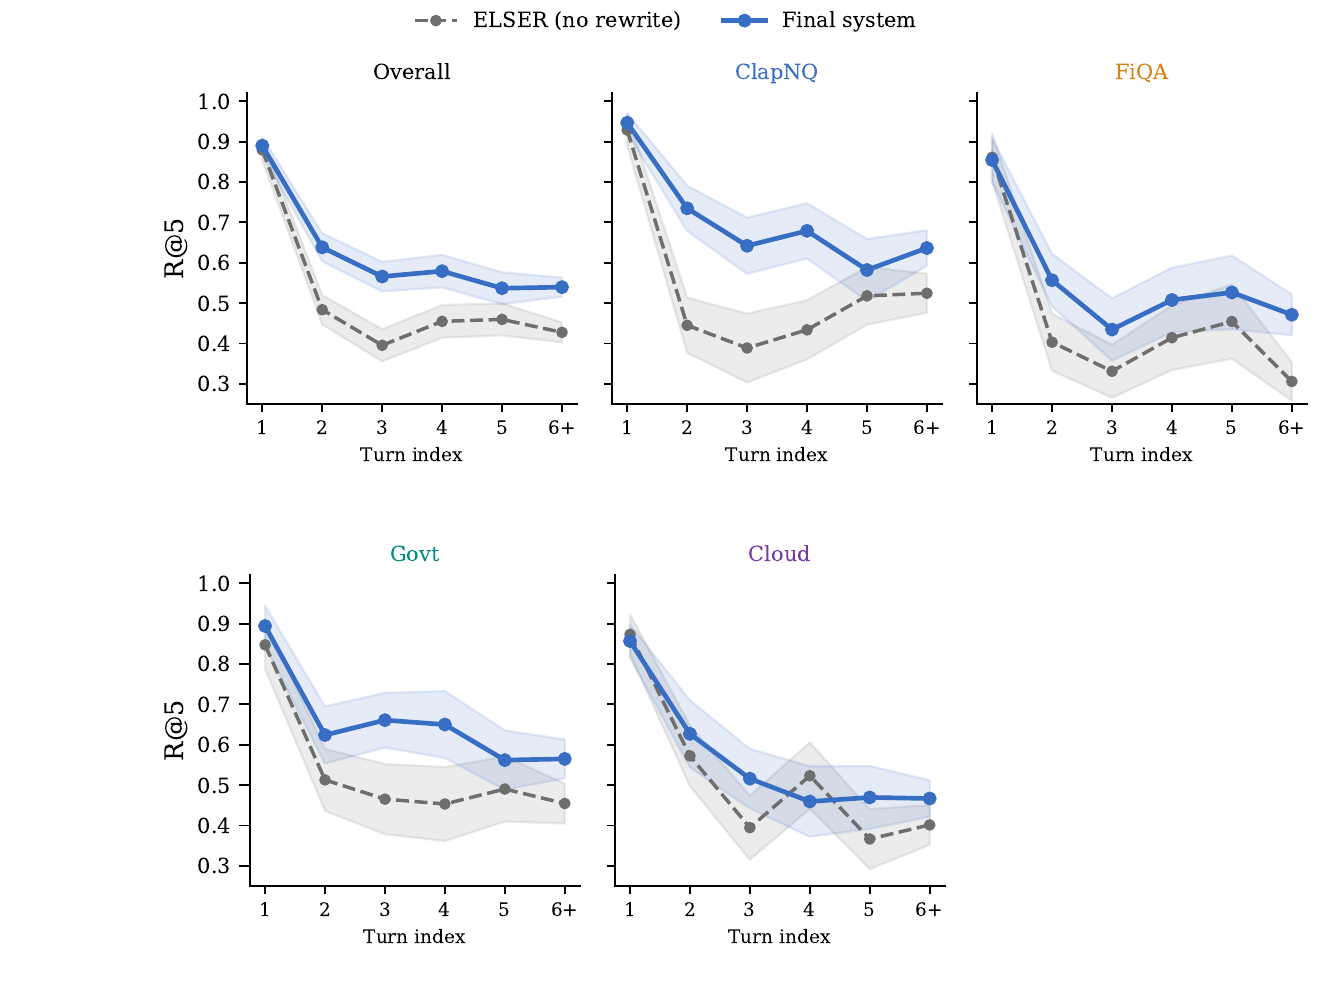
\includegraphics[width=\textwidth]{figures/fig8_turn_depth_domain_2rows.png}
\caption{Recall@5 by turn index, unaugmented ELSER baseline (dashed) vs.\ final system (solid), overall and per domain (shaded bands: $\pm 1$ standard error across conversations). Overall: Turn~1 $0.879$ and Turns~$6{+}$ $0.428$ for the baseline; Turn~1 $0.890$ and Turns~$6{+}$ $0.540$ for the final system.}
\label{fig:turn-depth-domain}
\end{figure}


\subsection{Rewriting Model Selection}
\label{sec:rewriting-model-selection}

The final system uses DeepSeek-V3.2 as the backbone for all five rewriting strategies
(Section~\ref{subsec:rewriting-engine}). This choice was validated against GPT-4o-mini and GPT-4o
across three representative strategies spanning the instruction-following--to--open-ended spectrum:
Minimal and Corpus-Specific (structured, schema-constrained outputs) and HyDE (open-ended
hypothetical-passage generation). Table~\ref{tab:rewriting-model-selection} reports Recall@5,
nDCG@5, and per-query cost for each combination.

\begin{table}[h]
\centering
\begin{tabular}{llccc}
\toprule
\textbf{Strategy} & \textbf{Model} & \textbf{R@5} & \textbf{nDCG@5} & \textbf{Cost/query} \\
\midrule
\multirow{3}{*}{Minimal}
 & DeepSeek-V3.2 (ours) & 0.527 & 0.487 & \$0.001 \\
 & GPT-4o-mini           & 0.513 & 0.481 & \$0.003 \\
 & GPT-4o                & 0.541 & 0.501 & \$0.015 \\
\midrule
\multirow{3}{*}{HyDE}
 & DeepSeek-V3.2 (ours) & 0.485 & 0.445 & \$0.001 \\
 & GPT-4o-mini           & 0.503 & 0.462 & \$0.003 \\
 & GPT-4o                & 0.504 & 0.464 & \$0.015 \\
\midrule
\multirow{3}{*}{Corpus-Specific}
 & DeepSeek-V3.2 (ours) & 0.541 & 0.498 & \$0.002 \\
 & GPT-4o-mini           & 0.517 & 0.479 & \$0.005 \\
 & GPT-4o                & 0.542 & 0.503 & \$0.020 \\
\bottomrule
\end{tabular}
\caption{Rewriting model comparison across strategy types (development set). GPT-4o's advantage
is concentrated on the open-ended HyDE strategy, at a 15$\times$ cost premium; on schema-constrained
strategies (Minimal, Corpus-Specific) DeepSeek-V3.2 is within $0.014$ R@5 of GPT-4o (no significance test was performed).}
\label{tab:rewriting-model-selection}
\end{table}

The pattern is not uniform across reformulation types. For strategies requiring strict instruction
following and structured JSON output — Minimal and Corpus-Specific — DeepSeek-V3.2 performs within
0.001--0.014 R@5 of GPT-4o, indicating that instruction-following capability, not raw generative
fluency, is the binding constraint for these tasks. GPT-4o's marginal advantage concentrates on
HyDE, where the task shifts from schema-constrained rewriting to open-ended hypothetical-passage
generation — a regime favoring stronger generative fluency. This gain (\,+0.019 R@5\,) is small in
absolute terms and arrives at a 15$\times$ cost premium; since HyDE is only one of five strategies
feeding into Nested RRF and is down-weighted at fusion (Table~\ref{tab:nested-rrf-weights-en}), the
quality delta does not justify the added expense. Notably, GPT-4o with Minimal rewriting matches
DeepSeek-V3.2 with Corpus-Specific (both R@5\,=\,0.541), suggesting model capability can partially
substitute for prompt specialization. We therefore retain DeepSeek-V3.2 across all five strategies
in the final system, consistent with the cost-efficiency principle underlying the model-routing
design of Section~\ref{sec:model-routing}.
%==============================================================
\subsection{Standalone vs.\ Non-Standalone Query Performance}
\label{sec:standalone-nonstandalone}

To isolate the mechanism behind the turn-depth degradation of Section~\ref{sec:turn-depth}, we
decompose Recall@5 by query type: \emph{standalone} queries (self-contained, no coreference
resolution needed) versus \emph{non-standalone} queries (dependent on prior turns).
Table~\ref{tab:standalone-nonstandalone} reports the unaugmented ELSER baseline against the final
system, both overall and per domain.

\begin{table}[h]
\centering
\begin{tabular}{lcccc}
\toprule
& \multicolumn{2}{c}{\textbf{ELSER (no rewrite)}} & \multicolumn{2}{c}{\textbf{Final system}} \\
\textbf{Domain} & SA & Non-SA & SA & Non-SA \\
\midrule
Overall & 0.879 & 0.440 & 0.890 & 0.564 \\
ClapNQ  & 0.929 & 0.477 & 0.946 & 0.651 \\
FiQA    & 0.861 & 0.363 & 0.854 & 0.493 \\
Govt    & 0.847 & 0.470 & 0.894 & 0.600 \\
Cloud   & 0.873 & 0.440 & 0.857 & 0.499 \\
\bottomrule
\end{tabular}
\caption{Recall@5 for standalone (SA) vs.\ non-standalone (Non-SA) queries, baseline vs.\ final
system. Rewriting improves Non-SA queries by $+12.4$ pp overall vs.\ only $+1.1$ pp for SA queries.}
\label{tab:standalone-nonstandalone}
\end{table}

\begin{figure}[h]
\centering
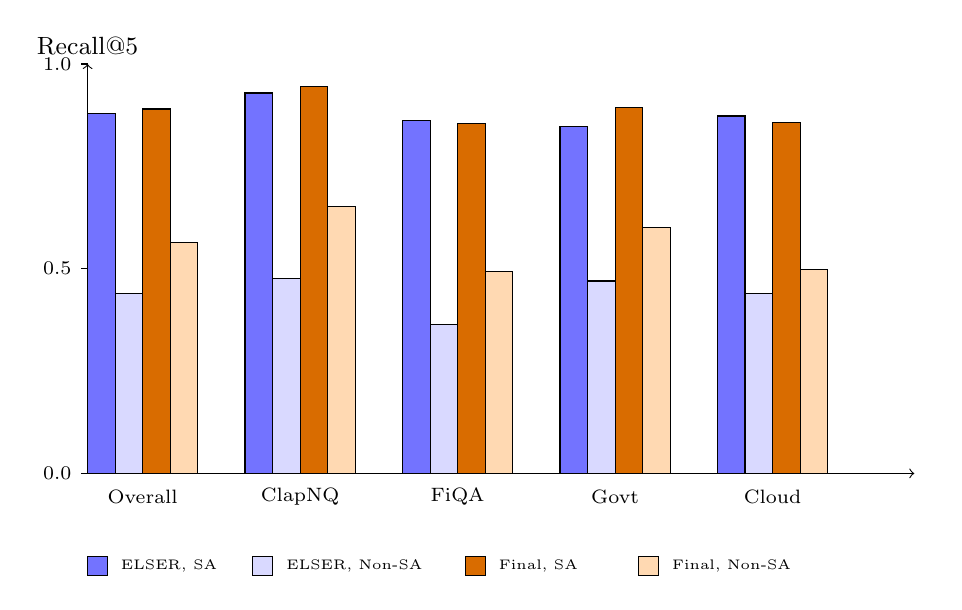
\begin{tikzpicture}
\begin{scope}
\draw[->] (0,0) -- (10.5,0) node[right, font=\small] {};
\draw[->] (0,0) -- (0,5.2) node[above, font=\small] {Recall@5};
\foreach \y/\lbl in {0/0.0, 2.6/0.5, 5.2/1.0}
  \draw (0,\y) -- (-0.08,\y) node[left, font=\scriptsize] {\lbl};
% Group layout: 5 domains x 4 bars (ELSER-SA, ELSER-NonSA, Final-SA, Final-NonSA), bar width 0.35, group width 2.0
\def\bw{0.35}
\def\gap{2.0}
\foreach \i/\dom/\esa/\ensa/\fsa/\fnsa in {
  0/Overall/4.567/2.288/4.628/2.933,
  1/ClapNQ/4.831/2.480/4.919/3.385,
  2/FiQA/4.477/1.888/4.441/2.564,
  3/Govt/4.404/2.444/4.649/3.120,
  4/Cloud/4.539/2.288/4.457/2.595}{
  \pgfmathsetmacro{\x}{\i*\gap}
  \draw[fill=blue!55] (\x,0) rectangle ++(\bw,\esa);
  \draw[fill=blue!15] (\x+\bw,0) rectangle ++(\bw,\ensa);
  \draw[fill=orange!85!black] (\x+2*\bw,0) rectangle ++(\bw,\fsa);
  \draw[fill=orange!30] (\x+3*\bw,0) rectangle ++(\bw,\fnsa);
  \node[font=\scriptsize] at (\x+2*\bw,-0.3) {\dom};
}
\end{scope}
\begin{scope}[yshift=-1.3cm, font=\tiny]
\draw[fill=blue!55] (0,0) rectangle ++(0.25,0.25); \node[right] at (0.3,0.12) {ELSER, SA};
\draw[fill=blue!15] (2.1,0) rectangle ++(0.25,0.25); \node[right] at (2.4,0.12) {ELSER, Non-SA};
\draw[fill=orange!85!black] (4.8,0) rectangle ++(0.25,0.25); \node[right] at (5.1,0.12) {Final, SA};
\draw[fill=orange!30] (7.0,0) rectangle ++(0.25,0.25); \node[right] at (7.3,0.12) {Final, Non-SA};
\end{scope}
\end{tikzpicture}
\caption{SA vs.\ Non-SA Recall@5 per domain for the ELSER baseline and the final system (values from Table~\ref{tab:standalone-nonstandalone}). Within each group the bars are, from left to right: ELSER SA (dark blue), ELSER Non-SA (light blue), final SA (dark orange), final Non-SA (light orange). The rewriting gain is concentrated on non-standalone queries; standalone performance is nearly unchanged.}
\label{fig:standalone-nonstandalone}
\end{figure}

The unaugmented baseline already achieves near-ceiling performance on standalone queries
(R@5\,=\,0.879), leaving little room for improvement — the $+0.011$ overall SA gain confirms that
query rewriting is not merely a generic retrieval booster, but a targeted fix for a specific failure
mode. The 43.9-percentage-point standalone/non-standalone gap in the unaugmented baseline directly
localizes the source of the drop after Turn~1 seen in Figure~\ref{fig:turn-depth-domain}: Turn~1
queries are standalone, while most later queries depend on earlier turns
(Section~\ref{sec:mtrag-corpus}), so the turn-position effect is largely a standalone-versus-non-standalone
effect rather than a gradual decay with depth. This finding supports Hypothesis H1
(Section~\ref{sec:rq}): the value of query rewriting lies in resolving conversational dependency,
not in improving retrieval quality uniformly. Rewriting slightly lowers standalone performance in
FiQA ($0.861 \rightarrow 0.854$) and Cloud ($0.873 \rightarrow 0.857$): unlike the Minimal and
Corpus-Specific prompts, which return standalone queries unchanged, the exploratory strategies
(HyDE, CoT, Anchor-Keyword) also reformulate standalone queries, and the added terms can displace
relevant passages. This cost is small compared with the non-standalone gains.

\subsubsection{Per-Domain Turn-Depth Degradation}
\label{sec:turn-depth-domain}

The per-domain panels of Figure~\ref{fig:turn-depth-domain} (Section~\ref{sec:turn-depth}) break the aggregate
turn-depth analysis down by domain, revealing that the 51\%$\to$39\% relative
degradation reduction reported for the overall corpus masks substantial domain heterogeneity. Cloud
and FiQA, the two domains with the highest lexical mismatch between conversational and document
language (Section~\ref{sec:mtrag-corpus}), retain the steepest late-turn drop even after
rewriting, while ClapNQ's encyclopedic phrasing is comparatively robust to dialogue depth.



The per-domain curves confirm the pattern anticipated from the corpus characterization of
Section~\ref{sec:mtrag-corpus}. ClapNQ, whose encyclopedic Wikipedia phrasing keeps lexical overlap
with the underlying documents high even under coreference, shows the largest rewriting gain at later
turns, and Table~\ref{tab:standalone-nonstandalone} shows the largest non-standalone gain of the four
domains ($0.477 \rightarrow 0.651$, $+17.4$ points). Cloud exhibits the noisiest
trajectory of the four domains, with the final system's curve crossing below the unaugmented
baseline around turn~4 before recovering; this instability is consistent with Cloud's technical,
identifier-heavy vocabulary (error codes, CLI flags, configuration keys), where a rewriting error
can introduce a plausible-looking but incorrect identifier rather than simply failing to resolve a
pronoun. Govt falls between these two extremes; like Cloud, FiQA retains a visible late-turn gap
relative to its own turn-1 performance even after rewriting, which is consistent with FiQA being
identified throughout this chapter (Section~\ref{sec:taskA-ablations}) as the structurally hardest
domain for retrieval regardless of turn depth. Overall, the per-domain breakdown does not
contradict the aggregate finding of Section~\ref{sec:turn-depth}, but it refines it: the 51\%$\to$39\%
relative-degradation reduction is not evenly distributed, and the residual late-turn gap that
rewriting fails to close is concentrated in the two domains with the largest vocabulary mismatch
between conversational and document language (Cloud and FiQA), rather than being a uniform property
of dialogue depth itself.

\section{Task B Generation Ablations and Component Contribution}
\label{sec:taskB-ablations}
%==============================================================

\subsection{Pipeline Component Ablation}

Table~\ref{tab:gen-ablation-en} decomposes the contribution of each stage of the Section~5.3 generation pipeline. The complete five-stage pipeline yields $+8.9$ Harmonic Mean points over single-pass greedy generation ($0.654 \rightarrow 0.743$), with evidence span extraction (Stage~2) contributing the single largest individual gain.

\begin{table}[h]
\centering
\small
\begin{tabular}{lc}
\toprule
\textbf{Pipeline Configuration} & \textbf{Harmonic Mean (HM)} \\
\midrule
Single Greedy Generation Baseline ($T{=}0.0$) & 0.654 \\
+ Verbatim Evidence Span Extraction & 0.688 \\
+ Dual-Candidate Drafting (Random Selection) & 0.706 \\
+ Technical Judge Verification & 0.725 \\
+ User Satisfaction Judge ($60\%$ stochastic sample) & 0.738 \\
+ Post-Processing Micro-Adjustments & \textbf{0.743} \\
\bottomrule
\end{tabular}
\caption{Task~B generation pipeline component contribution ablation, development set.}
\label{tab:gen-ablation-en}
\end{table}

Evidence span extraction alone accounts for $+0.034$ HM, together with a $+0.041$ gain in the reference-less faithfulness metric $RL_F$, consistent with the faithfulness part of Hypothesis~H2: constraining the generator's effective input to a compressed set of verbatim spans structurally bounds the space in which unsupported claims can be introduced.

\subsection{Extractiveness Band Calibration}

The extractiveness shaping function $\phi(r_4)$ of Equation~\eqref{eq:extractiveness-shaping} depends on a target band, set to $[0.28, 0.38]$ based on the empirical $4$-gram overlap of development-set reference answers ($36.2\%$ mean overlap). Table~\ref{tab:extractiveness-band-en} validates this choice against alternative bands: both tighter and looser bands score lower in HM than the selected configuration. The differences are small, so $[0.28, 0.38]$ is best read as the best of the bands tested rather than as a sharply defined optimum.

\begin{table}[h]
\centering
\small
\begin{tabular}{lcc}
\toprule
\textbf{Ideal Band} & \textbf{HM} & \textbf{$\Delta$ vs.\ ours} \\
\midrule
No shaping (uniform $\phi{=}0$) & 0.724 & $-0.019$ \\
$[0.20, 0.50]$ (loose) & 0.731 & $-0.012$ \\
$[0.25, 0.45]$ & 0.738 & $-0.005$ \\
\textbf{$[0.28, 0.38]$ (ours)} & \textbf{0.743} & --- \\
$[0.30, 0.40]$ (tight) & 0.737 & $-0.006$ \\
$[0.35, 0.50]$ (high) & 0.733 & $-0.010$ \\
\bottomrule
\end{tabular}
\caption{Extractiveness band sensitivity, development set. Deviation from $[0.28, 0.38]$ in either direction degrades HM.}
\label{tab:extractiveness-band-en}
\end{table}

\subsection{Model Routing}

The role-based routing of Section~\ref{sec:model-routing} is a cost-motivated design decision rather than an experimentally optimized one. At nominal API pricing, the routed Task~B pipeline costs an estimated \$0.010--0.012 per turn, of which the two GPT-4o generation calls account for \$0.009 (Table~\ref{tab:routing-en}); this is roughly $2$--$2.4\times$ less than the estimated \$0.024 for assigning GPT-4o to every stage. We did not retain a controlled comparison against uniform single-model configurations, and therefore make no claim about the effect of routing on output quality. The choice of DeepSeek-V3.2 for query rewriting is supported separately by the comparison of Section~\ref{sec:rewriting-model-selection}.

\subsection{Fixed Pipeline Settings}
\label{sec:additional-sweeps}

Two further settings of the Task~B pipeline were fixed by design rather than selected through a retained, systematic sweep: span extraction operates on at most five passages, and the User Satisfaction Judge is invoked on a random $60\%$ of turns as a compromise between judge coverage and API cost. We report them for reproducibility, without claiming that they are optimal.

%==============================================================
\section{Task C: Answerability Calibration as the Decisive Factor}
\label{sec:taskC-bottleneck}
%==============================================================

The end-to-end evaluation of Task~C shows a sharp drop relative to reference-grounded generation, with the global Harmonic Mean falling from $0.7698$ (Task~B) to $0.5409$ on the test set. Consistent with our system paper~\citep{athanasiou2026ailsntua}, we view answerability calibration as the decisive factor under the test distribution: the gate accepts most unanswerable turns even on the development set (Section~\ref{sec:pr-tradeoff}), and it was calibrated at an unanswerable rate of $6.5\%$ but faces $19.1\%$ at test time. Retrieval nonetheless remains a substantial factor. Task~C conditions generation on only the top-$3$ passages (Section~\ref{sec:e2e-system}), so top-rank precision ($R@5{=}0.607$ on the development set, Table~\ref{tab:ensemble-paradox-en}), rather than deep recall ($R@100{=}0.901$), determines whether the evidence reaches the generator; and top-$k$ retrieval errors account for most of the development-set failures inspected in Section~\ref{sec:error-analysis}, a split in which unanswerable turns are rare. A breakdown of the official test scores by answerability category would quantify the two contributions.

\subsection{The Precision--Recall Trade-off in Answerability Detection}
\label{sec:pr-tradeoff}

Across all gate configurations we evaluated, we observe a consistent trade-off: any attempt to increase the recall of \texttt{UNANSWERABLE} turns systematically decreases the recall of \texttt{ANSWERABLE} turns. Table~\ref{tab:answerability-en} shows that no evaluated configuration exceeds $25\%$ Unanswerable F1 on the full development set. Our full multi-judge system achieves $95.8\%$ recall on answerable turns but only $21.8\%$ recall on genuinely unanswerable turns---revealing a strong, systematic acceptance bias. Raw classification accuracy is deliberately not reported: with only $6.5\%$ unanswerable turns, a trivial always-answer policy would already exceed $93\%$ accuracy, making the metric uninformative for this decision. With only $55$ unanswerable turns in the development set, all of these estimates are coarse: the multi-judge recall of $21.8\%$ corresponds to $12$ turns (95\% Wilson interval $12.9$--$34.4\%$), the intervals of the two gated configurations overlap, and their difference in Unanswerable F1 ($24.0\%$ vs.\ $23.1\%$) amounts to a few turns.

\begin{table}[h]
\centering
\small
\begin{tabular}{lcccc}
\toprule
\textbf{Configuration} & \textbf{Ans.\ Recall} & \textbf{Unans.\ Recall [95\% CI]} & \textbf{Unans.\ Precision} & \textbf{Unans.\ F1} \\
\midrule
Always Answer Baseline & $100.0\%$ (777/777) & $0.0\%$ (0/55) & --- & $0.0\%$ \\
Pipeline + Verification Rule & $92.3\%$ (717/777) & $27.3\%$ (15/55) [17.3, 40.2] & $20.0\%$ (15/75) & $23.1\%$ \\
\textbf{Multi-Judge Voting Gate (Ours)} & \textbf{95.8\%} (744/777) & $21.8\%$ (12/55) [12.9, 34.4] & $26.7\%$ (12/45) & \textbf{24.0\%} \\
\bottomrule
\end{tabular}
\caption{Answerability detection on the development set ($N{=}832$ turns: $777$ answerable or partially answerable and $55$ unanswerable; the $10$ conversational turns are excluded). Intervals are 95\% Wilson score intervals. No gate configuration we evaluated exceeds $25\%$ Unanswerable F1 on the full development set.}
\label{tab:answerability-en}
\end{table}

The multi-judge gate improves end-to-end HM over a single-judge gate (Table~\ref{tab:taskC-ablation-en}) but does not remove this acceptance bias. Inspection of the gate's decisions suggests why: the document- and span-level judges often flag insufficient evidence, but the answer-level judge tends to accept drafted answers that remain plausible on their face, favoring fluency over evidentiary sufficiency. Removing the answer-level judge raised Unanswerable recall but lowered Answerable recall by rejecting partially supported, correct responses. These observations are qualitative; per-judge accuracies were not recorded, so we do not quantify the contribution of each judge.

\subsection{Error Analysis: Retrieval and Cross-Turn Dependency}
\label{sec:error-analysis}

To characterize Task~C failures, the author manually inspected $50$ failure cases from the development set and assigned each to one primary root cause (Table~\ref{tab:error-decomp-en}). The cases were not drawn by a documented random procedure and were labeled by a single annotator, so the percentages are indicative rather than precise estimates.

\begin{table}[h]
\centering
\small
\begin{tabular}{lcc}
\toprule
\textbf{Root Cause} & \textbf{\% of Failures} & \textbf{Primary Domain} \\
\midrule
Retrieval error (current-turn content) & $38\%$ & FiQA \\
Retrieval error (unresolved dependency on earlier turns) & $34\%$ & Cloud \\
Answerability misclassification & $18\%$ & All \\
Generation error (correct passages) & $10\%$ & ClapNQ \\
\bottomrule
\end{tabular}
\caption{Primary root cause in $50$ manually inspected Task~C failures (development set, single annotator). Retrieval-related causes account for $72\%$ of the inspected failures.}
\label{tab:error-decomp-en}
\end{table}

Retrieval-related causes together account for $72\%$ of the inspected failures, and answerability misclassification for $18\%$. The second retrieval category ($34\%$) requires a precise reading. Because MTRAGEval supplies the \emph{reference} conversation history rather than the system's own earlier outputs, an error made by our system at turn $t-1$ cannot propagate into $H_t$; the error cascade discussed in Section~3.3.2 is therefore not exercised by this evaluation. The $34\%$ category instead covers turns whose query depends on earlier turns and whose dependency the rewriting stage failed to resolve, so that retrieval at turn $t$ fails even though the history itself is correct. These cases point to coreference and ellipsis resolution as a major remaining retrieval weakness, consistent with the standalone/non-standalone gap of Section~\ref{sec:standalone-nonstandalone}.

\subsection{Threshold Sensitivity and the Task C Ablation}
\label{sec:task-c-ablation}

Table~\ref{tab:threshold-sweep-en} sweeps the answerability confidence threshold $\tau$ (Section~\ref{sec:e2e-system}) in $[0.5, 0.9]$, confirming that $\tau{=}0.7$ maximizes development-set HM by balancing Answerable recall against Unanswerable F1. This threshold was calibrated on a development set with only $6.5\%$ unanswerable turns, whereas the test set contains $19.1\%$. It is therefore plausibly miscalibrated for test conditions (Section~\ref{sec:leaderboard}); since we submitted a single frozen configuration, we cannot verify which threshold would have performed best on the test set.

\begin{table}[h]
\centering
\small
\begin{tabular}{lccc}
\toprule
\textbf{Threshold} & \textbf{HM} & \textbf{Answerable Recall} & \textbf{Unanswerable F1} \\
\midrule
0.50 & 0.573 & 0.892 & 0.261 \\
0.60 & 0.591 & 0.923 & 0.251 \\
\textbf{0.70 (ours)} & \textbf{0.610} & 0.958 & 0.240 \\
0.80 & 0.597 & 0.971 & 0.198 \\
0.90 & 0.578 & 0.986 & 0.162 \\
\bottomrule
\end{tabular}
\caption{Answerability confidence threshold sweep, development set. $\tau{=}0.70$ maximizes HM, but is calibrated against a development-set unanswerable rate roughly one-third of the test-set rate.}
\label{tab:threshold-sweep-en}
\end{table}

Finally, Table~\ref{tab:taskC-ablation-en} isolates the architectural decisions specific to the Task~C pipeline (Section~\ref{sec:e2e-system}). Adding an answerability gate yields the largest gain ($+0.043$ HM over always answering), replacing the single judge with the multi-judge gate adds $+0.025$, and reducing the retrieved passages from $5$ to $3$ adds a further $+0.024$, suggesting that in this self-retrieved setting additional, marginally relevant passages hurt more than they help.

\begin{table}[h]
\centering
\small
\begin{tabular}{lccc}
\toprule
\textbf{Configuration} & \textbf{HM} & \textbf{$RL_F$} & \textbf{$RB_{alg}$} \\
\midrule
Always answer (no gate) & 0.518 & 0.798 & 0.312 \\
Single-judge gate, top-5 passages & 0.561 & 0.821 & 0.356 \\
Multi-judge gate, top-5 passages & 0.586 & 0.836 & 0.383 \\
\textbf{Multi-judge gate, top-3 (ours)} & \textbf{0.610} & \textbf{0.848} & \textbf{0.408} \\
Multi-judge gate, top-1 & 0.591 & 0.841 & 0.389 \\
\bottomrule
\end{tabular}
\caption{Task~C ablation, development set. Rows change one setting at a time. The largest increment comes from adding a gate ($+0.043$ HM); the single-to-multi-judge and top-5-to-top-3 changes contribute $+0.025$ and $+0.024$. Top-1 underperforms top-3.}
\label{tab:taskC-ablation-en}
\end{table}

%==============================================================
\section{Official Competition Leaderboard Results}
\label{sec:leaderboard}
%==============================================================

The official, frozen leaderboard rankings for SemEval-2026 Task~8 support the design principles of Chapter~5 for retrieval and reference-grounded generation, while Task~C remains the weakest result. Table~\ref{tab:leaderboard-en} reports the complete official test-set results.

\begin{table}[h]
\centering
\small
\begin{tabular}{llccl}
\toprule
\textbf{Task} & \textbf{Metric} & \textbf{Ours} & \textbf{Rank} & \textbf{Top Baseline (Score)} \\
\midrule
A --- Retrieval & nDCG@5 & \textbf{0.5776} & \textbf{1/38} & ELSER + GPT-OSS-20b rewrite (0.4795) \\
B --- Generation & HM & 0.7698 & 2/26 & GPT-OSS-120b (0.6390) \\
C --- RAG & HM & 0.5409 & 11/29 & Qwen-30B-A3B-Thinking (0.5366) \\
\bottomrule
\end{tabular}
\caption{Official test set results. ``Top Baseline'' refers to the strongest non-participant system released by the organizers.}
\label{tab:leaderboard-en}
\end{table}

\begin{itemize}
    \item \textbf{Task~A (Retrieval Only):} the system ranks \textbf{1st out of 38} submissions with $\text{nDCG@5}{=}0.5776$, a $+20.5\%$ relative improvement over the strongest released baseline, consistent with Hypothesis~H1.
    \item \textbf{Task~B (Reference-Grounded Generation):} the system ranks \textbf{2nd out of 26} submissions with $\text{HM}{=}0.7698$ ($RB_{alg}{=}0.6327$, $RL_F{=}0.8971$, $RB_{llm}{=}0.8321$ on the individual components), narrowly behind the top-ranked system ($0.7827$), with particularly strong reference-less faithfulness and LLM-judged quality.
    \item \textbf{Task~C (End-to-End RAG):} the system ranks \textbf{11th out of 29} submissions with $\text{HM}{=}0.5409$, only marginally above the strongest organizer baseline ($0.5366$, $+0.004$). The Task~B$\rightarrow$C gap ($0.7698 \rightarrow 0.5409$) comes mostly from the drop in $RB_{alg}$ ($0.6327 \rightarrow 0.3998$). This drop is consistent with the answerability-calibration analysis of Section~\ref{sec:taskC-bottleneck}: the test set's near-tripled unanswerable rate ($19.1\%$ vs.\ $6.5\%$ at development time) leaves the development-calibrated threshold $\tau{=}0.7$ poorly matched to test conditions. Top-rank retrieval errors contribute as well, since only three retrieved passages reach the generator.
\end{itemize}

Because each subtask was evaluated with a single frozen configuration, the test set cannot confirm the individual component effects measured on the development set; it reports the performance of the complete systems only.

%==============================================================
\section{Synthesis: Answering the Research Questions}
\label{sec:eval-synthesis}
%==============================================================

We close this chapter by mapping each research question of Section~\ref{sec:rq} to the evidence reported above (Table~\ref{tab:rq-evidence}); the answers themselves are stated in Section~\ref{sec:rq-answers}.

\begin{table}[h]
\centering
\small
\begin{tabular}{p{0.07\textwidth}p{0.45\textwidth}p{0.38\textwidth}}
\toprule
\textbf{RQ} & \textbf{Evidence} & \textbf{Main caveat} \\
\midrule
RQ1 & Tables~\ref{tab:rewrite-ablation-en}, \ref{tab:reranking-alone-en}, \ref{tab:ensemble-paradox-en}; Sections~\ref{sec:turn-depth} and~\ref{sec:standalone-nonstandalone} & Pooling bias of the relevance labels (Section~\ref{sec:pooling-bias}); cumulative ablation \\
RQ2 & Tables~\ref{tab:gen-ablation-en} and~\ref{tab:extractiveness-band-en} & Development set only, single run per configuration \\
RQ3 & Tables~\ref{tab:answerability-en}, \ref{tab:threshold-sweep-en}, \ref{tab:taskC-ablation-en} and~\ref{tab:dev-test-en} & Only $55$ unanswerable development turns; one frozen test submission; no per-category test breakdown \\
RQ4 & Section~\ref{sec:taskA-ablations} (LLM reranking) & Low-weight interpolation gives marginal gains \\
\bottomrule
\end{tabular}
\caption{Evidence for each research question and its main limitation.}
\label{tab:rq-evidence}
\end{table}

Chapter~7 synthesizes these findings into the overall contributions of this thesis and discusses the concrete architectural limitations and future directions that follow from them.
